\chapter{量子ビット、複素状態ベクトル、そして観測量}

\lectureoverview{単一の電子スピンは、最初の真に量子力学的なビットである。それは任意の空間方向に対して準備されうるが、固定された検出器は二つの結果しか返さない。ここでは古典的な磁石の描像をいったん放棄し、実験が実際に行っていることを記述するために必要な複素ベクトル空間、確率規則、そして行列の言葉を構成する。}

\section{一つのスピンとベクトルの二つの意味}

古典的なビットは二つの可能な状態を持ち、その間に何もない。それらを\(0\)と\(1\)、表と裏、あるいは上と下と呼んでもよい。これらの名前は、古典的な状態空間における二つの異なる点につけられたラベルにすぎない。量子ビットもまた、固定された方法で測定すれば二つの選択肢を与えるが、二つの状態空間の点だけで記述することはできない。最も単純な例は電子のスピンである。

この例には二つの異なるベクトルの概念があり、それらを混同すると、これから先のすべてが不必要に不可解なものになる。第一に、通常の\emph{空間ベクトル}がある。すなわち、大きさと向きを持つ三次元空間内の矢印である。電子は磁気モーメントを持ち、当面の目的のためには、小さな磁石のように振る舞う。その大きさは固定されているが、準備の手続きによって空間的な向きをそれに割り当てることができる。

第二の対象は、複素ベクトル空間における抽象的なベクトルである。この\emph{状態ベクトル}が量子状態を記述することになる。それは単に磁気の矢印を別の記法で書き直したものではない。空間方向と状態ベクトルの関係は実在し重要であるが、それは二つの対象の同一性ではない。この関係は徐々に明らかにしていく。

\section{古典的描像を放棄する}

まず意図的に古典的な物語から始めよう。小さな磁石を強い外部磁場の中に置く。すでに整列していない限り、それは磁場のまわりで歳差運動をする。エネルギーを放射するにつれて歳差運動は減衰し、磁石は最低エネルギーの向きに落ち着く。印加磁場の向きを選び、この緩和を待ち、その後磁場を取り除くことによって、磁気モーメントを任意の望む向きに準備できるように思われる。

同じ装置は検出の方法も示唆する。選んだ向きに磁場をかけ、小さな磁石が落ち着く間に生じる放射を観測する。磁場に整列した古典的な磁石はエネルギーを放出しないはずである。最初に磁場と逆向きのものは最大量を放出し、中間の角度は中間の量を生じるはずである。その描像では、放射エネルギーは角度とともに連続的に変化する。

\begin{figure}[htbp]
\centering
\begin{coursefitfigure}
\begin{tikzpicture}[>=Latex,thick,scale=0.92]
  \draw[rounded corners] (-0.2,-0.2) rectangle (3.0,3.4);
  \node at (1.4,3.05) {\small preparation};
  \draw[->,very thick] (1.4,0.45) -- (1.4,2.55);
  \node[right] at (1.4,2.35) {\small applied field};
  \fill (1.4,1.35) circle (2.3pt);
  \draw[->,very thick] (1.4,1.35) -- (2.25,1.95);
  \node[below] at (1.4,0.15) {\small choose a direction and wait};

  \draw[->] (3.25,1.6) -- (4.25,1.6);

  \draw[rounded corners] (4.5,-0.2) rectangle (8.8,3.4);
  \node at (6.65,3.05) {\small measurement in a fixed direction};
  \draw[->,very thick] (5.15,0.45) -- (5.15,2.55);
  \fill (5.15,1.35) circle (2.3pt);
  \node[anchor=west] at (5.7,2.0) {no photon};
  \node[anchor=west] at (5.7,1.25) {one photon of fixed energy};
\node[anchor=west] at (5.7,0.5) {no intermediate outcome};
\end{tikzpicture}
\end{coursefitfigure}
\caption{操作上の難問。連続的に変化する準備の後に、二つの可能な出力しか持たない検出器が続く。}
\end{figure}

その古典的予言は電子に対しては誤りである。検出器の磁場をかけると、二つの結果しか生じない。
\begin{enumerate}
  \item 光子は放出されない。
  \item 下準位と上準位を分ける固定されたエネルギーを持つ光子が一つ放出される。
\end{enumerate}
そのエネルギーの任意の割合を運ぶ光子は決して存在しない。連続的な古典的応答は、二値的な量子の答えへと崩壊したのである。

準備に用いた向きが無関係になったわけではない。それは二つの答えの\emph{確率}を支配する。検出器に対して上向きに電子を準備すれば、上の結果が確実に生じる。下向きに準備すれば、遷移が確実に生じる。水平に準備すれば、垂直な検出器は二つの答えを同じ頻度で返す。
\begin{equation}
  P(\text{up})=\frac12,
  \qquad
  P(\text{down})=\frac12.
  \label{eq:l02-horizontal-probabilities}
\end{equation}
このように、連続的に変化する準備の族が、統計が連続的に変化する二値的な測定へとつながるのである。

\begin{classroomqa}
\lecturetimestamp{00:21:23}
\audiencequestion{巨視的な磁石の代わりに、別の小さな対象、おそらく第二の電子が磁場を供給することはできるだろうか。}
\lecturerresponse{それは可能であるが、その場合二つの電子は複合的な量子系を形成し、もつれ合うことがありうる。それこそがこの講義が向かう先である。一つの電子の状態空間を掌握するまで、それは保留する。}
\end{classroomqa}

\begin{classroomqa}
\lecturetimestamp{00:22:17}
\audiencequestion{確率分布は、準備と測定の全体を繰り返すことによって求めなければならないのか。同じ電子をもう一度測定するとどうなるのか。}
\lecturerresponse{はい、元の分布には、同一に準備された試行の繰り返しが必要である。最初の測定の後、その電子に対して同じ測定を繰り返すと同じ結果が得られる。測定はその検出器に対して電子を準備したのである。放射遷移を待つこと自体が、一つの可能な準備手続きである。}
\end{classroomqa}

\begin{classroomqa}
\lecturetimestamp{00:23:48}
\audiencequestion{自由電子を想定しているのか、それとも磁場は連続的に印加されたままなのか。}
\lecturerresponse{スピンの自由度だけを取り出し、電子の位置は、自由に運動していようと他の拘束を受けていようと無視する。大きな電磁石は、準備や検出のために素早くスイッチを入れられる。この簡略化された実験は、スピンについてのみ問うように設計されている。}
\end{classroomqa}

\begin{classroomqa}
\lecturetimestamp{00:25:22}
\audiencequestion{電子が正確に下向きに準備され、磁場が反転されたなら、光子は確実に放出されるのか、そしてそのエネルギーはどこから来るのか。}
\lecturerresponse{正確な反対向きの場合、遷移は確率1で起こる。斜めの準備の場合、確率はより小さい。エネルギーは究極的には外部磁場を確立または反転する際になされる仕事から来ており、装置もエネルギーの収支の一部である。}
\end{classroomqa}

\begin{classroomqa}
\lecturetimestamp{00:27:31}
\audiencequestion{光子はいつ現れるのか。遷移は瞬時なのか。}
\lecturerresponse{放出時刻は、不安定状態の崩壊時刻と同様にランダムである。特徴的な寿命や半減期を指定でき、より強い磁場はその尺度を短くする。エネルギー--時間の不確定性はより精密な記述に入り込むが、現在の操作的な事実は、二つの可能な出力とそれらの測定された頻度である。}
\end{classroomqa}

\begin{classroomqa}
\lecturetimestamp{00:29:17}
\audiencequestion{同一に準備された百万個の電子を含むビームは、単に測定可能な光の強度を生み出すだけなのか。}
\lecturerresponse{その通りである。集団の強度は平均的な遷移確率を明らかにするが、個々の電子の放出時刻は依然としてランダムである。集団は、単一の試行では示すことのできない分布を表示する。}
\end{classroomqa}

ここが出発点である。二つの孤立した古典的点は検出器の答えを符号化できるが、それらの答えの確率を変えるすべての準備を符号化することはできない。別の状態空間が必要である。

\section{複素数と状態空間の幾何学}

必要な状態空間は線形である。その要素は加算でき、スカラー倍できる。そのスカラーは複素数である。
\begin{equation}
  z=a+ib,
  \qquad
  i^2=-1,
  \qquad
  z^*=a-ib,
  \label{eq:l02-complex-number}
\end{equation}
ここで\(a\)と\(b\)は実数である。複素共役は正の量
\begin{align}
  z^*z
  &=(a-ib)(a+ib) \notag\\
  &=a^2+b^2.
  \label{eq:l02-complex-norm}
\end{align}
を生み出す。この単純な相殺が、確率規則の代数的な種である。

\begin{figure}[htbp]
\centering
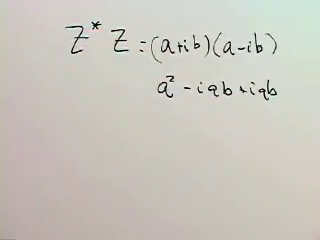
\includegraphics[width=0.74\linewidth]{lecture_02_figure_02.png}
\caption{複素共役と\(z^*z\)は、振幅が確率として解釈される前に黒板で展開される。}
\lectureframe{00:37:10}
\end{figure}

複素ベクトル空間は、\(c\)が複素数であるときはいつでも
\begin{equation}
  c\ket a,
  \qquad
  \ket a+\ket b
\end{equation}
が再びベクトルとなるような対象\(\ket a,\ket b,\ldots\)を含む。列ベクトルは具体的な実現を与える。
\begin{equation}
  \begin{aligned}
    \ket a&=
    \begin{pmatrix}
      a_1\\a_2\\ \vdots\\a_n
    \end{pmatrix},
    &
    c\ket a&=
    \begin{pmatrix}
      ca_1\\ca_2\\ \vdots\\ca_n
    \end{pmatrix},\\[0.7em]
    \ket a+\ket b&=
    \begin{pmatrix}
      a_1+b_1\\a_2+b_2\\ \vdots\\a_n+b_n
    \end{pmatrix}.
  \end{aligned}
  \label{eq:l02-vector-operations}
\end{equation}
複素数自身さえも一次元複素ベクトル空間をなす。電子スピンには二次元が必要である。

各列ケットに共役な行ブラを対応させる。
\begin{equation}
  \ket a=
  \begin{pmatrix}a_1\\a_2\end{pmatrix}
  \quad\longleftrightarrow\quad
  \bra a=
  \begin{pmatrix}a_1^*&a_2^*\end{pmatrix}.
  \label{eq:l02-bra-ket-components}
\end{equation}
このとき内積は
\begin{equation}
  \braket{b}{a}=b_1^*a_1+b_2^*a_2,
  \label{eq:l02-inner-product}
\end{equation}
であり、ノルムの二乗は
\begin{equation}
  \braket{a}{a}=|a_1|^2+|a_2|^2.
  \label{eq:l02-norm}
\end{equation}
である。すべての項が\(z^*z\)の形をしているので、これは実数で非負である。

\begin{classroomqa}
\lecturetimestamp{00:45:24}
\audiencequestion{なぜブラ記号に明示的なスターが付かないのか。}
\lecturerresponse{ケットをそのブラに変えることは、すでに転置と複素共役を意味している。ブラケットの反転はその操作の記法であり、もう一つスターを書くことは暗黙のうちに含まれていることを繰り返すことになる。}
\end{classroomqa}

\section{量子ビットの基底とボルンの規則}

ここで検出器に戻ろう。\(\ket{+}\)をその上状態、\(\ket{-}\)をその下状態とする。一般的なスピン状態は線形結合
\begin{equation}
  \ket\psi=a_+\ket{+}+a_-\ket{-}
  \quad\longleftrightarrow\quad
  \begin{pmatrix}a_+\\a_-\end{pmatrix}.
  \label{eq:l02-general-qubit}
\end{equation}
である。ケット内のプラスとマイナスの記号はラベルであり、算術演算ではない。この順序付けられた基底を選べば、
\begin{equation}
  \ket{+}=
  \begin{pmatrix}1\\0\end{pmatrix},
  \qquad
  \ket{-}=
  \begin{pmatrix}0\\1\end{pmatrix}.
  \label{eq:l02-basis-columns}
\end{equation}
実際、
\begin{equation}
  a_+\begin{pmatrix}1\\0\end{pmatrix}
  +a_-\begin{pmatrix}0\\1\end{pmatrix}
  =
  \begin{pmatrix}a_+\\a_-\end{pmatrix}.
  \label{eq:l02-basis-expansion}
\end{equation}

\begin{figure}[htbp]
\centering
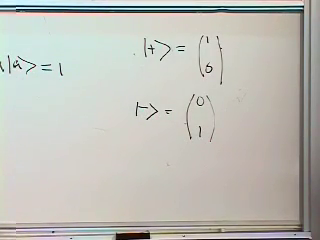
\includegraphics[width=0.72\linewidth]{lecture_02_figure_03.png}
\caption{検出器の状態は、二つの標準基底列として固定される。}
\lectureframe{00:58:10}
\end{figure}

係数は確率振幅である。各検出器結果の確率は、対応する振幅の大きさの二乗である。
\begin{equation}
  P(+)=|a_+|^2,
  \qquad
  P(-)=|a_-|^2.
  \label{eq:l02-born-rule}
\end{equation}
これらが唯一の結果であるから、
\begin{equation}
  \begin{gathered}
    |a_+|^2+|a_-|^2=1,\\
    \text{or equivalently}\qquad \braket{\psi}{\psi}=1.
  \end{gathered}
  \label{eq:l02-normalization}
\end{equation}
したがって、物理的な状態ベクトルは規格化されている。

\begin{classroomqa}
\lecturetimestamp{00:56:54}
\audiencequestion{プラスとマイナスの記号は成分において代数的な意味を持つのか。}
\lecturerresponse{ここではそれらは二つの基底状態とその係数をラベルする。それらを\(1\)と\(2\)、あるいは上と下と呼ぶこともできる。特に、\(-\ket{+}\)は\(\ket{+}\)の有効なスカラー倍であり、状態\(\ket{-}\)ではない。}
\end{classroomqa}

状態に絶対値1の複素数を掛けても、そのすべての確率は変わらない：
\begin{equation}
  \ket\psi\longmapsto e^{i\phi}\ket\psi,
  \qquad
  |e^{i\phi}a_\pm|^2=|a_\pm|^2.
  \label{eq:l02-global-phase}
\end{equation}
したがって、全体の位相だけが異なる2つのベクトルは同じ物理的状態を表す。\emph{相対}位相は別である。例えば\(a_-\)だけを\(-a_-\)に置き換える場合、ベクトル全体に1つの位相を掛けても一般には取り除けず、別の基底での測定結果を変えうる。

\begin{classroomqa}
\lecturetimestamp{00:59:54}
\audiencequestion{\(\ket{+}\)、\(-\ket{+}\)、\(e^{i\phi}\ket{+}\)は異なる状態か？重ね合わせの1つの項の符号を変える場合はどうか？}
\lecturerresponse{それらは異なる数学的ベクトルであるが、因子がベクトル全体に掛かり、その絶対値が1であるとき、それらは同じ物理的状態を記述する。上と下の項の間の相対的な符号または位相は、適切な測定において観測可能であり、したがって状態を変える。}
\end{classroomqa}

基底は正規直交である：
\begin{align}
  \braket{+}{+}&=1,
  &\braket{-}{-}&=1,
  \notag\\
  \braket{+}{-}&=0,
  &\braket{-}{+}&=0.
  \label{eq:l02-orthonormality}
\end{align}
例えば、
\begin{equation}
  \braket{+}{-}
  =
  \begin{pmatrix}1&0\end{pmatrix}
  \begin{pmatrix}0\\1\end{pmatrix}
  =0.
\end{equation}

\begin{figure}[htbp]
\centering
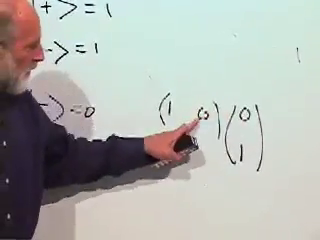
\includegraphics[width=0.76\linewidth]{lecture_02_figure_04.png}
\caption{上／下基底の4つの内積は黒板で直接確認される。}
\lectureframe{01:05:00}
\end{figure}

等重みの状態は、黒板での最初の有用な修正を与える。列
\begin{equation}
  \begin{pmatrix}1\\1\end{pmatrix}
\end{equation}
のノルムの二乗は\(2\)であり、\(1\)ではない。したがって規格化されていない。\(\sqrt2\)で割ることで修正される：
\begin{equation}
  \ket{\rightarrow}
  =
  \frac{1}{\sqrt2}
  \begin{pmatrix}1\\1\end{pmatrix}
  =
  \frac{\ket{+}+\ket{-}}{\sqrt2}.
  \label{eq:l02-horizontal-state}
\end{equation}
これは垂直検出器で\(P(+)=P(-)=1/2\)を与え、1つの水平準備に対応する。\((1,1)^T\)から\(2^{-1/2}(1,1)^T\)への修正は見かけ上のものではない。規格化こそが、振幅の二乗を完全な確率分布に変えるのである。

休憩の後、ベクトルの2つの意味に戻る価値がある。空間的な矢印は3つの実成分をもつ。量子ビットの状態ベクトルは2つの複素成分をもち、したがって規格化を課し全体の位相を同一視する前には4つの実数をもつ。これらの対象は関連しているが、一方が他方の単なる言い換えではない。それらの間の完全な幾何学的対応はまだ必要ない。

\begin{classroomqa}
\lecturetimestamp{01:10:56}
\audiencequestion{異なる量子系の状態空間の次元をどのようにして知るのか？}
\lecturerresponse{実験は、完全な測定が何個の相互に排他的な結果を区別できるかを教えてくれる。電子スピンにはそのような結果が2つあり、したがって2次元複素状態空間をもつ。スピン1の系は対応する測定において3つの結果をもち、3つの成分を必要とする。}
\end{classroomqa}

\section{古典的観測量とアンサンブル平均}

状態について述べたので、次に測定可能な量に移る。離散的な状態 \(n\) をもつ古典系において、可観測量はそれらの状態上の実数値関数 \(f_n\) である。状態が不確かであり、確率 \(p_n\) で記述されるなら、そのアンサンブル平均は
\begin{equation}
  \langle f\rangle_{\mathrm{ens}}
  =\sum_n p_n f_n.
  \label{eq:l02-classical-expectation}
\end{equation}
である。この記法は、1回の測定が必ずこの数に等しくなければならないということを意味するものではない。

コインに対して、\(f_+=+1\) と \(f_-=-1\) を割り当てる。すると
\begin{equation}
  \langle f\rangle_{\mathrm{ens}}
  =p_+-p_-.
  \label{eq:l02-coin-expectation}
\end{equation}
である。公正なコインでは平均はゼロである。\(p_+=3/4\) かつ \(p_-=1/4\) なら、平均は \(1/2\) である。\(0\) も \(1/2\) も1回の投げの結果ではなく、それぞれ多数の \(+1\) と \(-1\) の結果を要約したものである。

\begin{classroomqa}
\lecturetimestamp{01:23:30}
\audiencequestion{どちらの値も1回の試行には現れ得ないのに、期待値がゼロや2分の1になり得るのはなぜですか。}
\lecturerresponse{期待値という語は誤解を招きかねない。それは大きなアンサンブルの平均を意味し、次の試行で見るはずの値を意味するのではない。\(+1\) と \(-1\) の結果が公正な並びなら平均はゼロになり、3対1の偏りなら平均は2分の1になる。}
\end{classroomqa}

特に有用な観測量は、1つの状態に対する指示関数である：
\begin{equation}
  \chi_k(n)=
  \begin{cases}
    1,&n=k,\\
    0,&n\ne k.
  \end{cases}
\end{equation}
その平均は
\begin{equation}
  \langle\chi_k\rangle_{\mathrm{ens}}=p_k.
\end{equation}
したがって、すべての古典的観測量の平均を知ることは、特に確率分布を知ることを含む。

\section{行列と量子的観測量}

量子力学では、観測量は状態空間の点上の関数ではなく、線形演算子によって表される。有限次元状態空間では、それらの演算子は行列である。行列\(M\)は1つのベクトルを別のベクトルに写す：
\begin{equation}
  M\ket a=\ket{a'}.
  \label{eq:l02-matrix-action}
\end{equation}
2成分の場合、
\begin{equation}
  \begin{pmatrix}
    m_{11}&m_{12}\\
    m_{21}&m_{22}
  \end{pmatrix}
  \begin{pmatrix}a_1\\a_2\end{pmatrix}
  =
  \begin{pmatrix}
    m_{11}a_1+m_{12}a_2\\
    m_{21}a_1+m_{22}a_2
  \end{pmatrix}.
  \label{eq:l02-matrix-components}
\end{equation}

\begin{figure}[htbp]
\centering
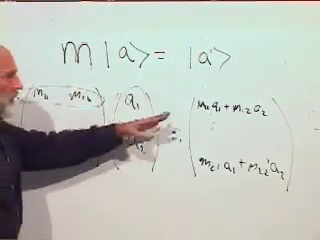
\includegraphics[width=0.78\linewidth]{lecture_02_figure_05.png}
\caption{行列の作用は、変換されたベクトルの2つの成分へ行ごとに展開される。}
\lectureframe{01:32:10}
\end{figure}

実二次元ベクトルは幾何学を可視化する。行列
\begin{equation}
  \begin{pmatrix}2&0\\0&2\end{pmatrix},
  \qquad
  \begin{pmatrix}1&0\\0&2\end{pmatrix},
  \qquad
  \begin{pmatrix}2&0\\0&1\end{pmatrix}
\end{equation}
はそれぞれ、すべての方向を一様に伸ばし、\(y\) 成分のみを伸ばし、\(x\) 成分のみを伸ばす。行列
\begin{equation}
  \begin{pmatrix}0&1\\1&0\end{pmatrix}
\end{equation}
は成分を入れ替え、平面を \(x=y\) に関して反射する。一方、
\begin{equation}
  \begin{pmatrix}0&1\\-1&0\end{pmatrix}
  \begin{pmatrix}v_x\\v_y\end{pmatrix}
  =
  \begin{pmatrix}v_y\\-v_x\end{pmatrix}
  \label{eq:l02-quarter-turn}
\end{equation}
は、黒板で用いた規約においてベクトルを時計回りに4分の1回転させる。せん断は別の線形な例を与えるが、その行列は練習問題として残す。本質的な制限は線形性である。平面の想像し得るすべての変換が行列で表されるわけではない。

量子可観測量は特別なクラスに属する。

\begin{definition}
行列\(M\)が\emph{エルミート}である条件は、次の等式が成り立つことである。
\begin{equation}
  M_{ij}=M_{ji}^*.
  \label{eq:l02-hermitian-condition}
\end{equation}
\end{definition}


対角条件 \(M_{ii}=M_{ii}^*\) は、すべての対角成分が実数であることを強制する。非対角成分は複素共役の対として現れる。例えば、
\begin{equation}
  M=
  \begin{pmatrix}
    r&4+i\\
    4-i&s
  \end{pmatrix},
  \qquad r,s\in\mathbb R,
  \label{eq:l02-hermitian-example}
\end{equation}
はエルミートである。すべての成分がたまたま実数なら、エルミートであることは対称であることと同じである。

\begin{figure}[htbp]
\centering
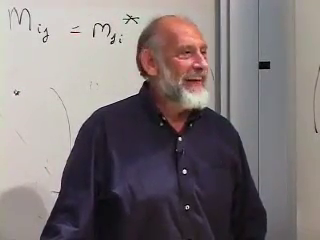
\includegraphics[width=0.75\linewidth]{lecture_02_figure_06.png}
\caption{対角線を挟んだ定義的な複素共役、\(M_{ij}=M_{ji}^*\) は、講義の最後に単独で扱う。}
\lectureframe{01:42:50}
\end{figure}

エルミート行列は、\(x\)、\(y\)、\(z\) 方向のスピンを含む測定可能な量を表す。これらは、物理的なキックや時間発展を記述する演算子と混同してはならない。

\begin{classroomqa}
\lecturetimestamp{01:45:49}
\audiencequestion{もし行列が状態を別の状態へキックするなら、それは規格化を保たなければならないのですか。エルミート行列はそれをしますか。}
\lecturerresponse{物理的なキックは状態ベクトルの長さを保たなければならないが、一般のエルミート行列はそうではない。長さを保つ変換はユニタリである。エルミート演算子は可観測量を表し、ユニタリ演算子は状態に作用する可逆な変換を表す。両者の詳しい関係は次に述べる。}
\end{classroomqa}

次の段階に必要な最小限の言語に到達した。量子ビットは2次元複素ベクトル空間における規格化されたベクトルであり、振幅が確率を定め、可観測量はエルミート行列である。これらの部品が揃ったので、任意方向のスピン、そして最終的にはもつれた対について、すでに破綻した古典的描像に戻ることなく議論できる。